% Anyon braiding worldlines — particle exchange in 2+1D spacetime (Ch 10)
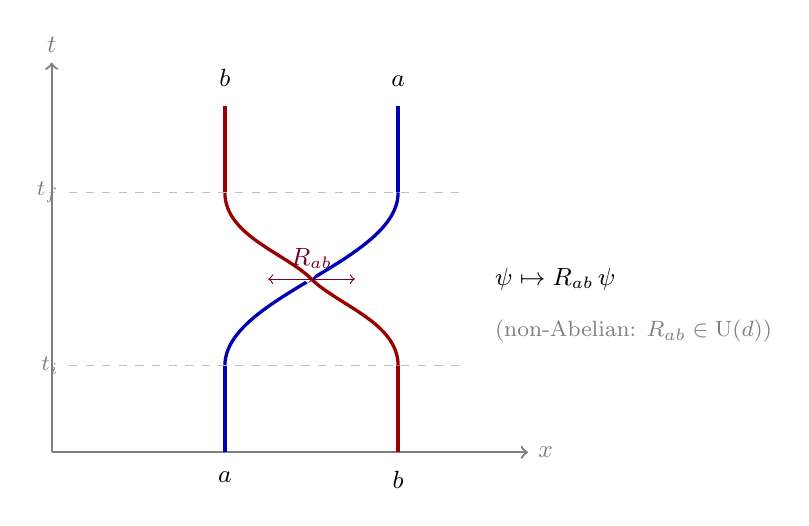
\begin{tikzpicture}[scale=1.1, thick,
    worldline/.style={very thick, blue!70!black},
    braid/.style={very thick, red!60!black}]

  % Time axis
  \draw[->, gray] (-0.5, 0) -- (-0.5, 4.5) node[above, font=\small] {$t$};

  % Spatial axis
  \draw[->, gray] (-0.5, 0) -- (5.0, 0) node[right, font=\small] {$x$};

  % Particle 1 worldline (goes right then left)
  \draw[worldline] (1.5, 0) -- (1.5, 1.0);
  \draw[worldline] (1.5, 1.0) .. controls (1.5, 1.8) and (3.5, 2.2) .. (3.5, 3.0);
  \draw[worldline] (3.5, 3.0) -- (3.5, 4.0);

  % Particle 2 worldline (goes left then right) — with crossing
  \draw[braid] (3.5, 0) -- (3.5, 1.0);
  % Under-crossing gap
  \draw[braid] (3.5, 1.0) .. controls (3.5, 1.5) and (2.8, 1.7) .. (2.5, 2.0);
  \draw[white, line width=4pt] (2.5, 2.0) .. controls (2.2, 2.3) and (1.5, 2.5) .. (1.5, 3.0);
  \draw[braid] (2.5, 2.0) .. controls (2.2, 2.3) and (1.5, 2.5) .. (1.5, 3.0);
  \draw[braid] (1.5, 3.0) -- (1.5, 4.0);

  % Particle labels
  \node[below, font=\small] at (1.5, -0.1) {$a$};
  \node[below, font=\small] at (3.5, -0.1) {$b$};
  \node[above, font=\small] at (3.5, 4.1) {$a$};
  \node[above, font=\small] at (1.5, 4.1) {$b$};

  % Braid annotation
  \draw[<->, thin, purple!60!black] (2.0, 2.0) -- (3.0, 2.0);
  \node[above, font=\small, purple!60!black] at (2.5, 2.0) {$R_{ab}$};

  % Phase annotation
  \node[right, font=\small] at (4.5, 2.0) {$\psi \mapsto R_{ab}\, \psi$};
  \node[right, font=\footnotesize, gray] at (4.5, 1.4) {(non-Abelian: $R_{ab} \in \mathrm{U}(d)$)};

  % Time slices
  \draw[dashed, thin, gray!50] (-0.3, 1.0) -- (4.3, 1.0);
  \draw[dashed, thin, gray!50] (-0.3, 3.0) -- (4.3, 3.0);
  \node[left, font=\footnotesize, gray] at (-0.3, 1.0) {$t_i$};
  \node[left, font=\footnotesize, gray] at (-0.3, 3.0) {$t_f$};
\end{tikzpicture}
